% \chapter{Discussion}
% \label{cha:discussion}
\chapter{Conclusion}
\label{cha:conclusion}

The focus of this report have been two-part. In the first part, methods for
vibration-based identification of localised nonlinearities have been explored and
validated. No assumption of the type of (localised) nonlinearity have been made, thus the
models works equally well for boundary, geometric, etc. types of nonlinearities.
Only stiffness have been treated; in theory the methods works just as well for
damping, but in practice damping is much harder due to the much smaller
magnitude and successful identification is still hard to obtain \autocite{noel2013a}.
Another subject that have been neglected, is identification using noisy
signals. The current FNSI implementation(in the vibration library) comes with
noise-weighting functions implemented as described by \autocite{noel2013a}(and
working accordingly to the description), but have not been tested en real noisy data.\\

In the second part, methods for investigating the behaviour of identified
nonlinear systems are treated. On the successful identification in part one, a
model is built and used for determine stability, bifurcations and internal
resonances. Where the methods in the first part requires some understanding and
knowledge about nonlinear system in order to obtain a good identification, the
methods here are easier to use and do not require as much knowledge (that said,
implementation wise they cannot be said to be easier).\\

One substantial lack in connecting the two parts, is the need to create a model
after identification is done. Current research are focused on eliminating this
step, and use the state space system identified by FNSI directly by the
numerical methods of the second part. Numerically this is
easy when both the FNSI and HB methods are implemented, but as shown in
\autocite{gourc2016a}, the FNSI method introduce spurious numerical
artefacts, and as long as these artefacts are present, the state space
formulation cannot be used directly. Preventing artefacts in the FNSI method
will be a big step forward in the seamless integration of the two methodologies.
Figure \ref{fig:fnsi_hb} shows the methodology.

\begin{figure}[!ht]
  \centering
  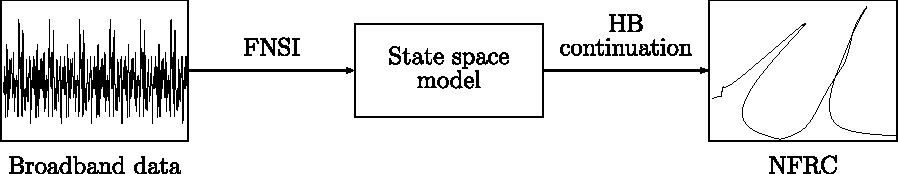
\includegraphics[width=0.7\linewidth]{discussion/fnsi_hb.pdf}
  \caption{FNSI-HB continuation procedure}
  \label{fig:fnsi_hb}
\end{figure}

This also concludes that focus have been on the methods, and efficient
implementation, and not application of them. The real limitations are not known
and using them on real life structures could be a complete project of it own.
For instance it have been assumed that a polynomial type of nonlinearity have a
integer order. This might not be case in real applications. FNSI can(or might) help
determine the polynomial order, but this have not been investigated.\\

Lacking in this thesis is the ability to track identified bifurcations.
This might be a potential feature in aiding designs: find the system parameters
where a bifurcation disappear. This could be exemplified as finding parameters
that prevents flutter. Bifurcation tracking is described in
\autocite{detroux2015a}. \\

As for the future of nonlinear system identification, progress have been made
within localised lumped nonlinearities - FNSI is just one of multiple methods - but
methods for distributed nonlinearities are still complicated and does not
convoy any physical interpretation due their flexible nature (ie. black box
models, where any combination of mathematical functions are mixed to model the
system.)\\



%%% Local Variables:
%%% mode: latex
%%% TeX-master: "../report"
%%% End:
